\documentclass[aspectratio=169, 11pt]{beamer}

% --- Plain, simple theme ---
\usetheme{default}
\usecolortheme{default}
\usefonttheme{professionalfonts}

% Clean navigation
\setbeamertemplate{navigation symbols}{}
\setbeamertemplate{footline}{%
  \hfill\insertframenumber/\inserttotalframenumber\hspace{1em}\vspace{0.5em}%
}

% Colours
\definecolor{ubblue}{RGB}{0, 76, 147}
\definecolor{ubgray}{RGB}{100, 100, 100}
\definecolor{lightgray}{RGB}{230, 230, 230}
\setbeamercolor{title}{fg=ubblue}
\setbeamercolor{frametitle}{fg=ubblue}
\setbeamercolor{structure}{fg=ubblue}
\setbeamercolor{block title}{bg=ubblue, fg=white}
\setbeamercolor{block body}{bg=lightgray}

% Packages
\usepackage[utf8]{inputenc}
\usepackage[T1]{fontenc}
\usepackage{amsmath}
\usepackage{booktabs}
\usepackage{graphicx}
\usepackage{tikz}
\usepackage{url}

% Compact itemize
\setbeamertemplate{itemize items}[circle]
\setbeamertemplate{enumerate items}[default]

% -------------------------------------------------------------------
% TITLE
% -------------------------------------------------------------------

\title{Data-Driven Cognitive Phenotyping\\in Acquired Brain Injury}
\subtitle{A Clustering Analysis with Imputation Robustness Assessment}
\author{Zolt\'an Kunos}
\institute{%
  MSc Fundamental Principles of Data Science\\
  Facultat de Matem\`atiques i Inform\`atica\\
  Universitat de Barcelona\\[0.5em]
  \textit{Supervisor:} Dr.\ Alejandro Garc\'ia-Rudolph%
}
\date{2025}

\begin{document}

% -------------------------------------------------------------------
\begin{frame}[plain]
  \maketitle
\end{frame}

% -------------------------------------------------------------------
% OUTLINE (~1 min)
% -------------------------------------------------------------------
\begin{frame}{Outline}
  \tableofcontents
\end{frame}

% ===================================================================
\section{Introduction}
% ===================================================================

% -------------------------------------------------------------------
\begin{frame}{Acquired Brain Injury: The Clinical Challenge}
  \begin{itemize}
    \item \textbf{ABI} includes TBI, stroke, hypoxic injury, encephalitis
    \item Leading cause of long-term disability in working-age adults
    \item Cognitive effects span attention, memory, executive function, language, visuoperception
    \item \textbf{Key problem:} similar injury severity $\to$ very different cognitive profiles
  \end{itemize}

  \vspace{1em}
  \begin{block}{Why it matters}
    Severity bands and diagnostic labels group patients with substantively different cognitive profiles together, and the within-group variation that could guide treatment is hidden.
  \end{block}
\end{frame}

% -------------------------------------------------------------------
\begin{frame}{Research Questions \& Hypotheses}
  \begin{columns}[T]
    \begin{column}{0.5\textwidth}
      \textbf{Research Questions}
      \begin{enumerate}
        \item Does clustering find \textbf{distinct cognitive phenotypes}?
        \item Are phenotypes \textbf{stable} across imputation methods?
        \item Does cluster membership \textbf{link to clinical unit}?
        \item Does \textbf{domain-level} clustering beat variable-level?
      \end{enumerate}
    \end{column}
    \begin{column}{0.5\textwidth}
      \textbf{Formal Hypotheses}
      \begin{description}
        \item[H1] $\geq 2$ phenotypes, Silhouette $> 0.40$, noise $< 30\%$
        \item[H2] Pairwise ARI $> 0.50$ across imputation methods
        \item[H3] $\chi^2$ significant, Cram\'er's $V > 0.10$
        \item[H4] Domain wins all 3 metrics: Silhouette, VIF, cond.\ number
      \end{description}
    \end{column}
  \end{columns}
\end{frame}

% ===================================================================
\section{Data \& Methods}
% ===================================================================

% -------------------------------------------------------------------
\begin{frame}{Dataset Overview}
  \begin{columns}[T]
    \begin{column}{0.55\textwidth}
      \begin{itemize}
        \item Raw extract: \textbf{22,075 assessments}, \textbf{8,739 patients}
        \item Single neurorehabilitation centre
        \item 31 original columns (25 cognitive + 6 admin)
        \item Routine clinical data
        \item Large \& systematic missingness
      \end{itemize}

      \vspace{0.5em}
      \textbf{Tier~1 Filtering} (50\% threshold + $\geq 1$ cognitive test):
      \begin{itemize}
        \item \textbf{14 eligible variables}, \textbf{6 cognitive domains}
        \item \textbf{17,406 assessments} from \textbf{7,285 patients}
      \end{itemize}

      \vspace{0.5em}
      \textbf{Complete-case analysis:}
      \begin{itemize}
        \item Only \textbf{9,245} rows (\textbf{53.1\%}) have all 14 tests
        \item Listwise deletion discards \textbf{46.9\%} of data
        \item $\Rightarrow$ Imputation is essential
      \end{itemize}
    \end{column}
    \begin{column}{0.45\textwidth}
      \centering
      \small
      \begin{tabular}{l c}
        \toprule
        \textbf{Domain} & \textbf{Vars} \\
        \midrule
        Orientation        & 3 \\
        Attention          & 2 \\
        Visuoperception    & 1 \\
        Language           & 3 \\
        Memory             & 4 \\
        Executive Function & 1 \\
        \midrule
        \textbf{Total}     & \textbf{14} \\
        \bottomrule
      \end{tabular}
    \end{column}
  \end{columns}
\end{frame}

% -------------------------------------------------------------------
\begin{frame}{Imputation Methods: A 5-Category Taxonomy}

  \small
  \begin{table}
    \centering
    \begin{tabular}{l l}
      \toprule
      \textbf{Category} & \textbf{Methods} \\
      \midrule
      Conventional Statistical & Mean, EM, MICE \\
      Machine Learning         & KNN, MissForest \\
      Hybrid                   & Predictive Mean Matching (PMM) \\
      Matrix Completion        & SoftImpute, NMF \\
      Deep Learning            & Denoising Autoencoder, Variational Autoencoder \\
      \bottomrule
    \end{tabular}
  \end{table}

  \vspace{0.5em}
  \begin{itemize}
    \item Extends Afkanpour et al.\ (2024) 4-category taxonomy $\to$ adds \textbf{Deep Learning}
    \item DAE: 15$\to$128$\to$64$\to$32$\to$64$\to$128$\to$15, \textbf{pattern-aware} corruption 0.2, 5 runs averaged
    \item VAE: same architecture, latent dim = 32, \textbf{cyclical} $\beta$: $0 \to 0.1$, $K = 20$ samples averaged
    \item \textbf{10 methods $\times$ 2 representations} = 20 pipeline runs
  \end{itemize}
\end{frame}

% -------------------------------------------------------------------
\begin{frame}{Deep Learning Improvements}
  \begin{columns}[T]
    \begin{column}{0.5\textwidth}
      \textbf{DAE: Pattern-Aware Corruption}
      \begin{itemize}
        \item Standard: corrupt random 20\% of values
        \item Problem: real missingness is \textbf{structured} (tests given together)
        \item Solution: 50\% of corruption masks sampled from empirical co-occurrence patterns
        \item Result: DAE learns from realistic missing patterns
      \end{itemize}
    \end{column}
    \begin{column}{0.5\textwidth}
      \textbf{VAE: Cyclical $\beta$-Annealing}
      \begin{itemize}
        \item Standard: fixed $\beta = 0.1$ on KL term
        \item Problem: \textbf{posterior collapse} --- latent space ignored early in training
        \item Solution: $\beta$ ramps $0 \to 0.1$ over 40-epoch cycles
        \item Result: better latent space + reconstruction
      \end{itemize}

      \vspace{0.5em}
      \textbf{Held-out RMSE:} 10\% holdout evaluation confirms DAE outperforms VAE on all variables
    \end{column}
  \end{columns}
\end{frame}

% -------------------------------------------------------------------
\begin{frame}{Method Comparison at a Glance}
  \small
  \centering
  \begin{tabular}{l l c c c l}
    \toprule
    \textbf{Category} & \textbf{Method} & \textbf{Year} & \textbf{Sil.} & \textbf{$k$} & \textbf{Key Strength} \\
    \midrule
    Conv.\ Stat. & Mean & --- & 0.604 & 4 & Simplest baseline \\
                 & EM & 1977 & 0.587 & 4 & MLE under normality \\
                 & MICE & 2011 & 0.598 & 3 & Gold standard; flexible \\
    \midrule
    Machine Learning & KNN & 2001 & 0.576 & 4 & Non-parametric; local \\
                     & MissForest & 2012 & 0.606 & 3 & Non-linear; mixed types \\
    \midrule
    Hybrid & PMM & --- & 0.498 & 4 & Preserves distribution \\
    \midrule
    Matrix Compl. & SoftImpute & 2010 & 0.571 & 4 & Efficient; regularised \\
                  & NMF & 1999 & 0.546 & 3 & Non-negativity natural \\
    \midrule
    Deep Learning & DAE & 2018 & 0.510 & 5 & Deep non-linear \\
                  & VAE & 2014 & 0.603 & 4 & Probabilistic uncertainty \\
    \bottomrule
  \end{tabular}

  \vspace{0.5em}
  Methods span 1977--2018. $k$ = clusters from HDBSCAN; Sil.\ = silhouette score.
\end{frame}

% -------------------------------------------------------------------
\begin{frame}{Analysis Pipeline: UMAP + HDBSCAN}
  \centering
  \resizebox{0.95\textwidth}{!}{%
  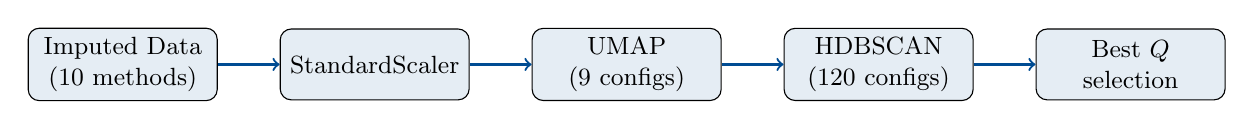
\begin{tikzpicture}[
    box/.style={draw, rounded corners, fill=ubblue!10, minimum width=2.4cm, minimum height=0.9cm, align=center, font=\small},
    arr/.style={->, thick, ubblue}
  ]
    \node[box] (imp) at (0,0) {Imputed Data\\(10 methods)};
    \node[box] (std) at (3.2,0) {StandardScaler};
    \node[box] (umap) at (6.4,0) {UMAP\\(9 configs)};
    \node[box] (hdb) at (9.6,0) {HDBSCAN\\(120 configs)};
    \node[box] (sel) at (12.8,0) {Best $Q$\\selection};

    \draw[arr] (imp) -- (std);
    \draw[arr] (std) -- (umap);
    \draw[arr] (umap) -- (hdb);
    \draw[arr] (hdb) -- (sel);
  \end{tikzpicture}%
  }

  \vspace{1em}
  \begin{columns}[T]
    \begin{column}{0.5\textwidth}
      \textbf{UMAP grid:}
      \begin{itemize}
        \item \texttt{n\_neighbors}: 15, 30, 50
        \item \texttt{min\_dist}: 0.0
        \item \texttt{n\_components}: 3, 5, 8
      \end{itemize}
    \end{column}
    \begin{column}{0.5\textwidth}
      \textbf{HDBSCAN grid:}
      \begin{itemize}
        \item \texttt{min\_cluster\_size}: 500--3000
        \item \texttt{min\_samples}: 5, 10, 25, 50
        \item \texttt{method}: eom, leaf
        \item \texttt{epsilon}: 0.0, 0.1, 0.5
      \end{itemize}
    \end{column}
  \end{columns}

  \vspace{0.5em}
  \centering
  $Q = \text{Silhouette} \times (1 - \text{noise proportion})$\\[0.3em]
  \small + Reliability-weighted domains, RobustScaler, consensus UMAP (10 seeds), KNN noise reassignment
\end{frame}

% -------------------------------------------------------------------
\begin{frame}{Shared Pipeline Design for H2}
  \begin{block}{Problem}
    Many moving parts vary across methods: scaling, UMAP embedding, cluster boundaries.
  \end{block}

  \vspace{0.5em}
  \textbf{Solution --- isolate the imputation effect:}
  \begin{enumerate}
    \item Fit StandardScaler on \textbf{MICE} $\to$ \texttt{transform()} all others
    \item Fit UMAP on \textbf{MICE} $\to$ \texttt{transform()} all others
    \item Fit $K$-Means on \textbf{MICE embedding} $\to$ \texttt{predict()} all others
  \end{enumerate}

  \vspace{0.5em}
  \begin{itemize}
    \item Same $k$, same boundaries, same embedding geometry
    \item \textbf{Only source of variation:} the imputed values themselves
    \item HDBSCAN labels retained for H1/H3/H4; $K$-Means labels for H2
  \end{itemize}
\end{frame}

% ===================================================================
\section{Results}
% ===================================================================

% -------------------------------------------------------------------
\begin{frame}{Clustering Results Across Imputation Methods}
  \small
  \centering
  \begin{tabular}{l c c c c}
    \toprule
    \textbf{Method} & \textbf{Clusters} & \textbf{Silhouette} & \textbf{Noise \%} & \textbf{Clustered $N$} \\
    \midrule
    Mean       & 4 & 0.604 &  3.3 & 16,832 \\
    KNN        & 4 & 0.576 &  7.3 & 16,135 \\
    MICE       & 3 & 0.598 &  7.8 & 16,048 \\
    MissForest & 3 & 0.606 & 14.4 & 14,899 \\
    PMM        & 4 & 0.498 &  4.1 & 16,692 \\
    EM         & 4 & 0.587 &  7.4 & 16,118 \\
    SoftImpute & 4 & 0.571 & 16.9 & 14,464 \\
    NMF        & 3 & 0.546 & 12.4 & 15,248 \\
    DAE        & 5 & 0.510 &  4.3 & 16,657 \\
    VAE        & 4 & 0.603 & 16.6 & 14,516 \\
    \bottomrule
  \end{tabular}

  \vspace{0.5em}
  \begin{itemize}
    \item Cluster count ranges from 3 to 5 across methods (primary MICE: 3 tiers)
    \item Silhouette on the HDBSCAN core (pre-reassignment); the final full-coverage MICE solution scores \textbf{0.526}
    \item Best UMAP: \texttt{n\_components=8}; HDBSCAN: \texttt{min\_cluster\_size=1000, min\_samples=50, eom}
  \end{itemize}
\end{frame}

% -------------------------------------------------------------------
\begin{frame}{H1: Discrete, Stable Clusters --- \textcolor{green!60!black}{Supported}}
  \begin{columns}[T]
    \begin{column}{0.55\textwidth}
      \textbf{Per-method bootstrap (50 iters):}
      \begin{itemize}
        \item \textbf{10 / 10} methods clear pre-registered thresholds\\
          (median silhouette $>$ 0.40, pre-KNN noise $<$ 0.30)
        \item Cluster count 3--5 across methods (MICE: 3)
      \end{itemize}

      \vspace{0.4em}
      \textbf{Per-cluster core Jaccard (Hennig):}
      \begin{itemize}
        \item Above-Average: \textbf{0.63}, Global Impairment: \textbf{0.62}
        \item Near-Normal (middle band): 0.47
      \end{itemize}

      \vspace{0.4em}
      \textbf{Three severity tiers} (a severity gradient, not dissociated profiles):
      \begin{description}\small
        \item[Above-Average] ($n = 6{,}725$): above cohort mean on all domains
        \item[Near-Normal] ($n = 6{,}328$): near the cohort average
        \item[Global Impairment] ($n = 4{,}353$): below cohort mean on all domains
      \end{description}
    \end{column}
    \begin{column}{0.45\textwidth}
      \begin{block}{Verdict}
        \textbf{Supported}\\[0.3em]
        10 / 10 methods clear sil + noise thresholds (pre-registered: $\ge 8/10$)\\[0.3em]
        PC1 = 56\% of variance: the cohort sits on a single overall-severity axis.
      \end{block}
    \end{column}
  \end{columns}
\end{frame}

% -------------------------------------------------------------------
\begin{frame}{H2: Imputation Robustness --- \textcolor{green!60!black}{Supported}}
  \scriptsize \textit{ARI is chance-corrected concordance: 0 = random, 1 = perfect. 0.50 = substantial overlap; 0.90+ = near-identical clusterings.}\\[0.3em]
  \begin{columns}[T]
    \begin{column}{0.55\textwidth}
      \textbf{Shared pipeline:}
      \begin{itemize}
        \item Mean pairwise ARI: \textbf{0.710} \\
              \quad \textit{95\% bootstrap CI [0.704, 0.716]}
        \item Every one of the 45 pairs exceeds 0.50 (range 0.51--0.88)
        \item Consensus confidence: \textbf{0.929}; high-confidence assessments: \textbf{86.2\%}
      \end{itemize}

      \vspace{0.5em}
      \textbf{Holm-corrected pairwise tests:}\\
      \textbf{44 / 45} pairs reject $H_0{:}\,\text{ARI}\!\le\!0.5$\\
      Only \textbf{KNN--SoftImpute} (0.509) borderline.
    \end{column}
    \begin{column}{0.45\textwidth}
      \textbf{Top ARI pairs:}
      \begin{itemize}
        \item EM--DAE: 0.880
        \item DAE--VAE: 0.863
        \item EM--VAE: 0.828
      \end{itemize}

      \vspace{0.5em}
      \textbf{Instability correlation:}\\
      $r = 0.474$ (per-assessment vs.\ missing fraction)

      \vspace{0.3em}
      \textbf{Takeaway:} the severity tiers survive every imputation choice; MICE is a safe default.
    \end{column}
  \end{columns}
\end{frame}

% -------------------------------------------------------------------
\begin{frame}{H3: Clinical Unit Association --- \textcolor{green!60!black}{Supported}}
  \begin{itemize}
    \item $\chi^2 = 911.3$, $p \approx 4 \times 10^{-156}$
    \item Cram\'er's $V = 0.162$
    \item Rubin-pooled ($M{=}5$ MICE): $V = 0.154$ [0.049, 0.259]
    \item \textbf{CMH test:} association \textbf{not confounded} by diagnosis group
  \end{itemize}

  \vspace{0.5em}
  \begin{block}{Interpretation}
    \begin{itemize}
      \item Small effect size (Cohen), but well above the 0.10 threshold
      \item Association \textbf{holds after stratifying by diagnosis} --- not a confound
      \item Severity tier adds explanatory power beyond diagnosis; supports severity-informed routing
    \end{itemize}
  \end{block}
\end{frame}

% -------------------------------------------------------------------
\begin{frame}{H4: Domain vs.\ Variable Level --- \textcolor{green!60!black}{Supported}}
  \small
  \textbf{Rule:} Domain wins if it beats variable-level on the three quality metrics:\\
  \quad higher Silhouette, lower mean VIF, lower condition number.

  \vspace{0.5em}
  \begin{columns}[T]
    \begin{column}{0.5\textwidth}
      \centering
      \begin{tabular}{l c c c}
        \toprule
        \textbf{Metric} & \textbf{Domain} & \textbf{Variable} & \textbf{Winner} \\
        \midrule
        Silhouette   & \textbf{0.481} & 0.473  & Domain   \\
        Mean VIF     & \textbf{1.88}  & 2.77   & Domain   \\
        Cond.\ number & \textbf{11.8}  & 61.7   & Domain   \\
        \bottomrule
      \end{tabular}

      \vspace{0.5em}
      Domain wins \textbf{all three} metrics.
    \end{column}
    \begin{column}{0.5\textwidth}
      \textbf{Why domain-level wins:}
      \begin{enumerate}
        \item \textbf{Comparable separation:} silhouette 0.481 vs 0.473
        \item \textbf{Less multicollinearity:} VIF 2.77 $\to$ 1.88, condition number 61.7 $\to$ 11.8
        \item \textbf{More interpretable:} clinicians think in domains, not individual tests
      \end{enumerate}
    \end{column}
  \end{columns}
\end{frame}

% -------------------------------------------------------------------
\begin{frame}{Hypothesis Summary}
  \centering
  \begin{tabular}{l l l}
    \toprule
    \textbf{Hypothesis} & \textbf{Verdict} & \textbf{Key Evidence} \\
    \midrule
    H1: Discrete, stable clusters & \textcolor{green!60!black}{Supported} & 10/10 methods pass sil/noise; 3 severity tiers \\
    H2: Imputation robustness & \textcolor{green!60!black}{Supported} & ARI = 0.710, 44/45 Holm-significant \\
    H3: Clinical unit assoc. & \textcolor{green!60!black}{Supported} & $\chi^2 = 911$, $V = 0.162$, CMH not confounded \\
    H4: Domain vs.\ variable & \textcolor{green!60!black}{Supported} & Domain wins all 3 metrics (sil, VIF, cond.) \\
    \bottomrule
  \end{tabular}
\end{frame}

% -------------------------------------------------------------------
\begin{frame}{Robustness Additions}
  \small
  \begin{columns}[T]
    \begin{column}{0.5\textwidth}
      \textbf{A-3: Bootstrap 95\% CIs}
      \begin{itemize}\small
        \item H2 mean ARI: 0.710 [0.704, 0.716]
        \item H3 Cram\'er's $V$: 0.16 [0.15, 0.18]
        \item H4 silhouette gap: 0.05 [0.04, 0.06]
      \end{itemize}

      \vspace{0.3em}
      \textbf{A-2: Holm for 45 H2 pairs}
      \begin{itemize}\small
        \item \textbf{44 / 45} pairs reject ARI${\le}0.5$
        \item Only KNN--SoftImpute borderline
      \end{itemize}

      \vspace{0.3em}
      \textbf{A-4: Rubin-pooled ($M{=}5$ MICE)}
      \begin{itemize}\small
        \item Cram\'er's $V = 0.154$ [0.049, 0.259]
        \item H4 gap $= 0.050$ [0.043, 0.058]
      \end{itemize}
    \end{column}
    \begin{column}{0.5\textwidth}
      \textbf{A-5: Listwise-deletion baseline}
      \begin{itemize}\small
        \item Complete cases: 9{,}245 / 17{,}406
        \item \textbf{2 clusters} (vs 3 in MICE)
        \item Silhouette 0.257 (vs 0.526)
        \item ARI vs MICE $= 0.625$
        \item[$\Rightarrow$] Imputation materially changes structure
      \end{itemize}

      \vspace{0.3em}
      \textbf{D-1: Outcome-adjacent (TSI + within-patient)}
      \begin{itemize}\small
        \item TSI by tier: 214 / 188 / 172 d (Kruskal--Wallis $p{=}4e{-}28$)
        \item \textbf{50.2\%} of multi-assessment patients stay in same tier
        \item Transitions move \emph{up} the gradient (recovery) 3:1
      \end{itemize}
    \end{column}
  \end{columns}
\end{frame}

% ===================================================================
\section{Discussion}
% ===================================================================

% -------------------------------------------------------------------
\begin{frame}{Key Findings \& Interpretation}
  \begin{enumerate}
    \item \textbf{A cognitive severity gradient, not dissociated phenotypes:} 3 tiers (Above-Average / Near-Normal / Global Impairment); PC1 = 56\% of variance, all domains co-vary
    \item \textbf{No attention-specific dissociation} --- PC1 (56\%) loads near-equally on all six domains; the tiers differ in overall level, not profile shape
    \item \textbf{Imputation matters:} listwise deletion finds 2 clusters (sil 0.257) vs.\ 3 with MICE (sil 0.53)
    \item \textbf{H2 survives correction:} 44 of 45 pairs pass Holm; every pair exceeds ARI 0.50
    \item \textbf{Severity tier is not diagnosis:} CMH not confounded; adds independent explanatory power
    \item \textbf{Cautionary tale:} the apparent attention phenotype was a preprocessing artefact (a mis-scaled demographic) --- it dissolved under correction
  \end{enumerate}
\end{frame}

% -------------------------------------------------------------------
\begin{frame}{Clinical Implications}
  \begin{columns}[T]
    \begin{column}{0.5\textwidth}
      \textbf{Match intensity to severity:}
      \begin{itemize}
        \item Above-Average $\to$ vocational rehab, community return
        \item Global Impairment $\to$ intensive, structured rehabilitation
      \end{itemize}

      \vspace{0.5em}
      \textbf{Decision support:}
      \begin{itemize}
        \item CogDash dashboard classifies new patients
        \item Shows confidence for each assignment
      \end{itemize}
    \end{column}
    \begin{column}{0.5\textwidth}
      \textbf{Method recommendations:}
      \begin{itemize}
        \item Use MICE as default for clinical neuropsych data
        \item Test sensitivity with $\geq 2$ imputation methods
        \item Prefer domain-level features for clustering
        \item Report stability/confidence alongside phenotype labels
      \end{itemize}
    \end{column}
  \end{columns}
\end{frame}

% -------------------------------------------------------------------
\begin{frame}{Interactive Dashboard: CogDash}
  \begin{columns}[T]
    \begin{column}{0.55\textwidth}
      \textbf{8 modules:}
      \begin{enumerate}
        \item Home --- summary metrics \& hypothesis verdicts
        \item Cluster Explorer --- t-SNE 2D \& UMAP 3D
        \item Cognitive Profiles --- radar charts \& heatmaps
        \item Patient Lookup --- individual patient profiles
        \item Imputation Comparison --- ARI/NMI matrices
        \item Clinical Units --- cross-tabulations
        \item New Patient Classification --- decision support
        \item Advanced Analytics --- feature importance, stability
      \end{enumerate}
    \end{column}
    \begin{column}{0.45\textwidth}
      \textbf{Tech stack:}
      \begin{itemize}
        \item Streamlit + Plotly interactive plots
        \item Colour-blind safe palette
        \item Docker containerised
        \item Pre-computed results (pickle)
      \end{itemize}
    \end{column}
  \end{columns}
\end{frame}

% ===================================================================
\section{Limitations \& Future Work}
% ===================================================================

% -------------------------------------------------------------------
\begin{frame}{Limitations \& Mitigations}
  \small
  \begin{enumerate}
    \item \textbf{Single-centre} --- but tests (TMT, Stroop, digit span) are \textbf{internationally standard} for 30+ years
    \item \textbf{A continuum, not natural kinds} --- the tiers discretise a single severity axis; tier count (3--5) depends on resolution
    \item \textbf{Feature-engineering sensitivity} --- the earlier attention phenotype was an artefact of a mis-scaled demographic; corrected by winsorise + sign-align + standardise
    \item \textbf{MAR assumption} --- but 10-method comparison + Rubin pooling + listwise baseline act as built-in sensitivity analyses
    \item \textbf{No functional outcome variables} --- D-1 is only outcome-adjacent (TSI, within-patient stability)
    \item \textbf{Cross-sectional} --- but multiple assessments per patient give coverage of the recovery continuum (recovery direction confirmed)
  \end{enumerate}
\end{frame}

% -------------------------------------------------------------------
\begin{frame}{Future Directions}
  \begin{itemize}
    \item \textbf{Longitudinal phenotyping} --- track cognitive change over recovery
    \item \textbf{Multi-centre validation} --- test reproducibility across settings
    \item \textbf{Recovery prediction} --- use phenotype as a prognostic tool
    \item \textbf{Advanced imputation} --- GANs (GAIN), transformers for larger batteries
    \item \textbf{Neuroimaging integration} --- link phenotypes to brain structure/function
  \end{itemize}
\end{frame}

% ===================================================================
\section{Conclusions}
% ===================================================================

% -------------------------------------------------------------------
\begin{frame}{Conclusions}
  \begin{enumerate}
    \item \textbf{A cognitive severity gradient in ABI:} 3 tiers (Above-Average / Near-Normal / Global Impairment) on a single severity axis (PC1 56\%), cutting across diagnostic categories
    \item \textbf{Imputation is not cosmetic:} listwise deletion recovers 2 clusters (sil 0.257) vs.\ 3 with MICE (sil 0.53); ARI 0.625 between the two
    \item \textbf{Robust across imputation:} 44 of 45 H2 pairs survive Holm; every pair exceeds ARI 0.50
    \item \textbf{Domain-level features beat} variable-level on all three quality metrics (silhouette, VIF, condition number), confirmed via Rubin pooling
    \item \textbf{Severity tier adds clinical value} beyond diagnosis (CMH not confounded); 86% of assessments get high-confidence labels
  \end{enumerate}

  \vspace{1em}
  \begin{block}{Methodological Contribution}
    An imputation-robustness framework for clustering, \emph{plus} a worked cautionary case: preprocessing artefacts can masquerade as cognitive phenotypes unless features are scaled and screened with care.
  \end{block}
\end{frame}

% -------------------------------------------------------------------
\begin{frame}[plain]
  \centering
  \vspace{2cm}
  {\LARGE\textcolor{ubblue}{Thank you}}\\[1.5em]
  {\large Questions?}\\[2em]
  \textcolor{ubgray}{Zolt\'an Kunos}\\
  \textcolor{ubgray}{Universitat de Barcelona}\\[0.8em]
  \textcolor{ubgray}{z.kunos@gmail.com}\\[1em]
  \small\textcolor{ubgray}{Code \& dashboard: \url{https://github.com/zkunos/thesis_project}}
\end{frame}

\end{document}
